% ==============================================================================
% CAPÍTULO 3 - METODOLOGIA
% ==============================================================================

\chapter{Metodologia}
\label{cap:metodologia}

O desenvolvimento do projeto Oficina Master adotou uma abordagem metodológica pragmática e adaptada à realidade de um projeto conduzido por um único desenvolvedor. Em vez de replicar frameworks projetados para equipes — como Scrum ou SAFe —, optou-se por um processo autogerenciado, orientado à entrega de funcionalidades completas e verticalmente integradas, fundamentado no uso do sistema de controle de versão \textit{Git} e guiado por uma visão de produto definida pelo gestor responsável.

\section{Definição de Escopo e Visão de Produto}

O ponto de partida do processo metodológico foi uma etapa de alinhamento estratégico entre o gestor do projeto e o desenvolvedor. Nessa fase, o gestor apresentou a visão geral do sistema — seus objetivos de negócio, os módulos essenciais e as prioridades de alto nível —, sem a necessidade de especificações formais exaustivas ou documentação de requisitos completa de antemão.

Essa transferência de visão ocorreu por meio de conversas diretas e objetivas, nas quais o desenvolvedor absorveu o contexto do problema, fez perguntas pontuais de esclarecimento e, a partir disso, conduziu de forma autônoma o detalhamento técnico de cada funcionalidade. Conforme destacado por \citeonline{pressman}, em projetos de menor escala e com equipes reduzidas, a comunicação direta e a autonomia técnica do desenvolvedor tendem a substituir com vantagem os rituais formais de cerimônias ágeis.

\section{Fluxo de Desenvolvimento Orientado a \textit{Features}}

Em substituição ao modelo de entrega baseado em ciclos fixos de tempo (\textit{Sprints}), adotou-se um modelo orientado a funcionalidades completas. Cada unidade de trabalho correspondia a uma \textit{feature} funcional do sistema — um módulo ou comportamento coeso e testável de ponta a ponta — que só era considerado concluído quando estivesse integralmente implementado, do banco de dados à interface do usuário.

Esse modelo apresentou vantagens práticas relevantes para o contexto do projeto:

\begin{itemize}
    \item Eliminação da pressão artificial de prazos semanais, permitindo que funcionalidades complexas — como o mecanismo de \textit{Tenant Switching} e a camada de autenticação de \textit{APIs} — recebessem o tempo necessário para uma implementação robusta;
    \item Entregas sempre em estado funcional e utilizável, facilitando a validação incremental pelo gestor ao final de cada módulo concluído;
    \item Maior clareza sobre o progresso real do projeto, uma vez que o critério de conclusão era objetivo: a funcionalidade funciona ou não funciona.
\end{itemize}

O sequenciamento das \textit{features} foi definido com base em suas dependências técnicas e na prioridade de negócio indicada pelo gestor. Módulos centrais da arquitetura foram desenvolvidos primeiro, estabelecendo uma base sólida sobre a qual as funcionalidades periféricas puderam ser construídas com segurança.

\section{Controle de Versão com \textit{Git}}

O \textit{Git} foi utilizado como ferramenta central de controle de versão e rastreabilidade do trabalho realizado. A estratégia de ramificação adotada foi simples e adequada ao contexto de desenvolvedor solo: para cada nova funcionalidade, criava-se uma \textit{branch} dedicada a partir do ramo principal, onde todo o desenvolvimento era realizado de forma isolada. Ao término e validação local da \textit{feature}, o código era integrado ao ramo principal por meio de um \textit{merge} direto.

Essa abordagem garantiu:

\begin{itemize}
    \item Histórico de desenvolvimento limpo e organizado por funcionalidade, facilitando eventuais reversões ou análises futuras;
    \item Isolamento seguro entre funcionalidades em desenvolvimento simultâneo, mesmo que conduzidas pelo mesmo desenvolvedor em momentos distintos;
    \item Rastreabilidade direta entre commits e as funcionalidades às quais se referem, por meio de mensagens de commit descritivas e padronizadas.
\end{itemize}

O histórico de contribuições documenta a evolução incremental da base de código, conforme demonstrado na \autoref{fig:github_repo} e na \autoref{fig:git_log}, refletindo o rigor aplicado no versionamento do projeto.

\begin{figure}[htb]
    \caption{\label{fig:github_repo}Visão Geral do Repositório no GitHub e Histórico de Sincronização}
    \centering
    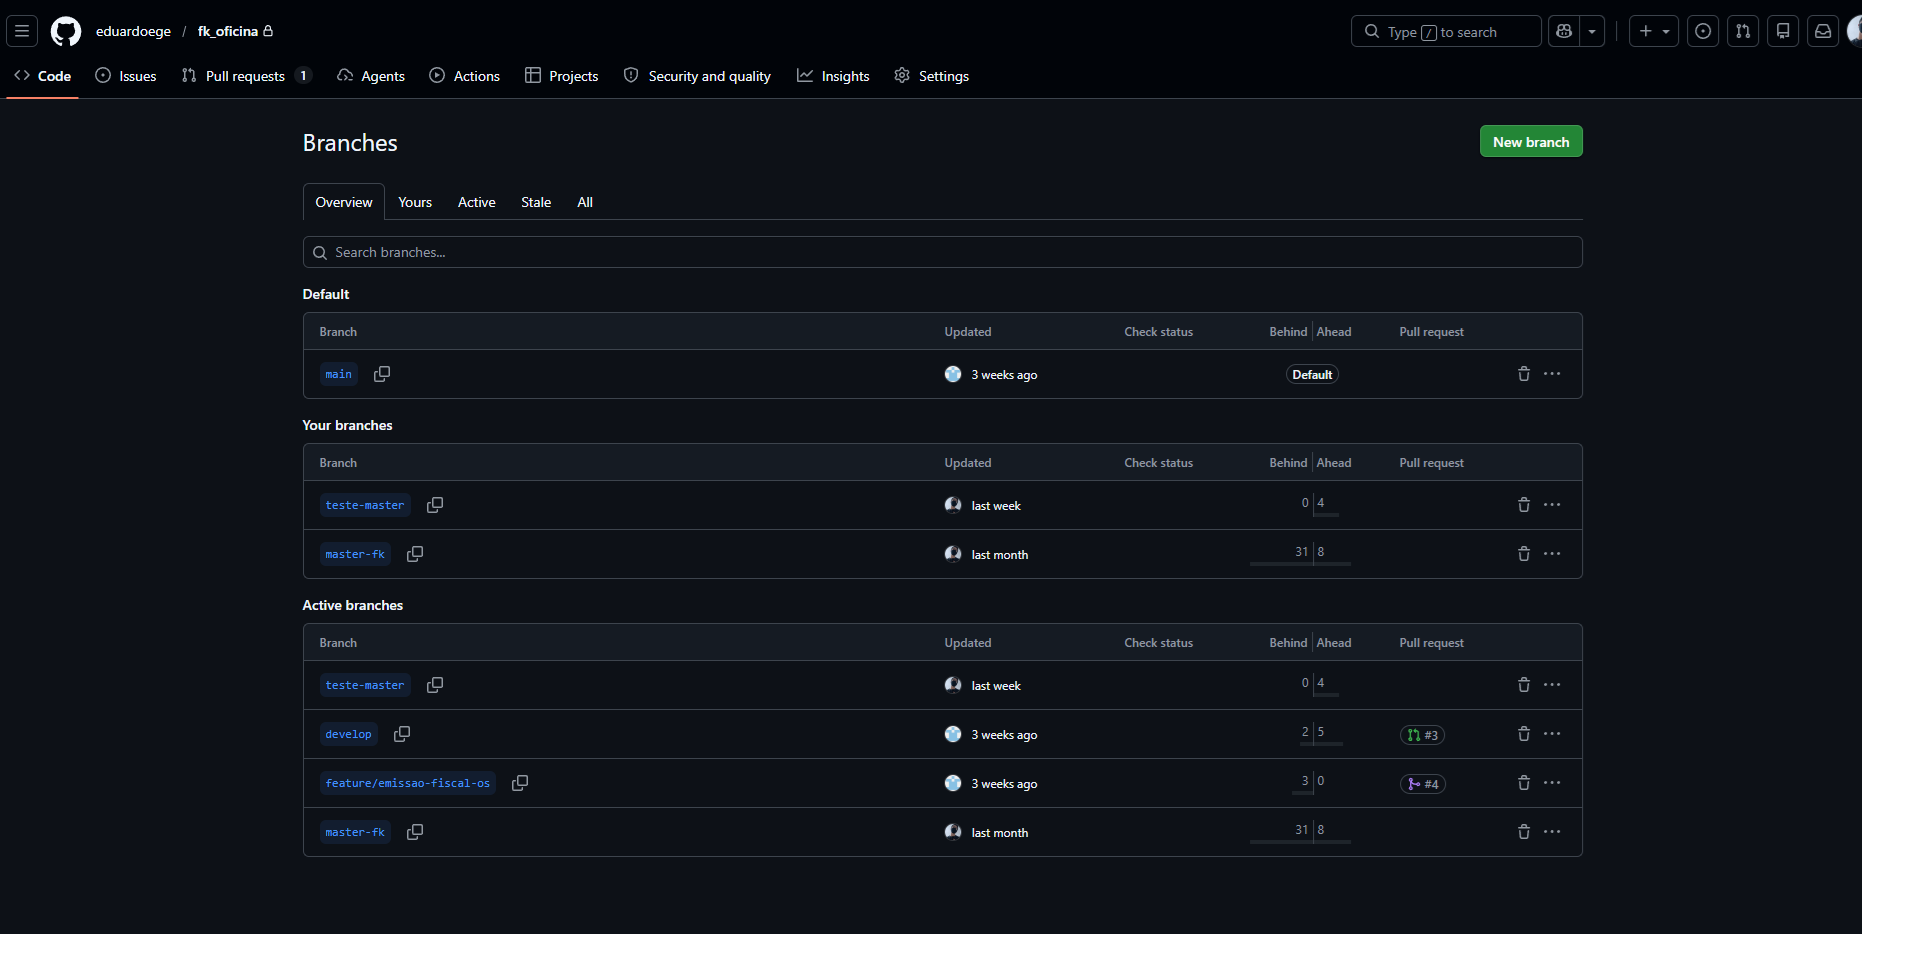
\includegraphics[width=0.8\textwidth]{figuras/05-desenvolvimento/github.png}
    \legend{Fonte: Própria do autor (2026).}
\end{figure}

\begin{figure}[htb]
    \caption{\label{fig:git_log}Histórico de Contribuições e Versionamento do Projeto}
    \centering
    \begin{lstlisting}[language=bash]
* b87b445 gerenciamento dos usuarios do master
* a67b8d6 update licenca e plano
* 374cdb0 UPDATE INTEGRACAO MASTER COM OFICINA
* 567aeb4 teste master
* dd7abfa Release: Modulo Fiscal completo + clonagem NF-e
* 7092d15 Merge pull request #2 from eduardoege/develop
* 615c231 Merge branch 'develop' of fk_oficina
* 66ed4bc Merge branch 'feature/emissao-fiscal-os'
* ff3ffb3 fix(fiscal): exibe PDF e bloqueia transmissao
* 98b998f feat(fiscal): clonar NF-e e suporte a origem clone
* f8d4761 feat(master): registra logs de login
    \end{lstlisting}
    \legend{Fonte: Própria do autor (2026).}
\end{figure}

Não foram adotadas práticas de \textit{Code Review} por pares nem esteiras formais de integração contínua, uma vez que a natureza individual do projeto tornava tais práticas desnecessárias. A qualidade do código foi assegurada pela disciplina do próprio desenvolvedor, pelo uso de ferramentas de análise estática e pela validação funcional a cada entrega.

\section{Validação e Alinhamento Contínuo}

Ao final do desenvolvimento de cada \textit{feature}, realizava-se uma breve sessão de validação com o gestor. Nesse momento, a funcionalidade era demonstrada em ambiente local ou de homologação, coletavam-se eventuais ajustes ou redirecionamentos e definia-se informalmente a próxima funcionalidade a ser desenvolvida.

Esse ciclo curto de \textit{feedback} — sem a burocracia de cerimônias formais — permitiu manter o alinhamento entre a visão de produto do gestor e as decisões técnicas do desenvolvedor ao longo de todo o projeto, garantindo que cada entrega agregasse valor real e mensurável ao sistema.

Esta metodologia, embora desprovida de cerimônias formais, demonstrou-se eficaz e adequada ao perfil do projeto: ágil na comunicação, disciplinada no versionamento e focada na entrega de valor funcional a cada iteração.